\documentclass{article}
\usepackage[utf8]{inputenc}
\usepackage[numbers,sort&compress]{natbib}
\usepackage{hyperref}
\usepackage{todonotes}
\usepackage{graphicx}
\usepackage{subfig}
\usepackage{amsmath}
\usepackage[toc,page]{appendix}
\usepackage{amssymb}
%\usepackage{gensymb}
\usepackage{soul}
\usepackage{placeins}

\title{Direct detection of dark matter}
\author{Peter Bosch, Max Briel and Jelle van Urk}
\date{June 2018}

\graphicspath{ {Images/} }

\begin{document}

\maketitle

Recommended article for programming:

https://arxiv.org/pdf/1002.1912.pdf

Review article about whole DM searches (including direct detection): \cite{Roszkowski:2017nbc}.

More theoretical: \cite{Queiroz:2017kxt}.

Probing WIMP particle physics and astrophysics with direct detection and neutrino telescope data:
https://arxiv.org/pdf/1410.8051.pdf

\section{Introduction}


- Observational clues for the presence of Dark Matter (Go more into this) 
Deviations from the galactic rotation curves and other astrophysical observations provide evidence for the presence of additional unobserved matter: Dark Matter. From the Cosmic Microwave background it has been deduced that this matter cannot be of baryonic nature and accounts for 63\% of the matter in the universe [REFERENCE], while only interacting gravitationally with ordinary matter. 
This lead to the idea of the WIMP particle, a Weakly Interacting Massive Particle, as an source of observed gravitational interactions. 
However, since its only weakly interacting with ordinary matter, its detection is a difficult task. This can either be achieved using a indirect detection, where products that can only come from Dark Matter interactions are observed. However, the possibility remains for other processes to give the same results. 

More concrete evidence can be provided by direct detection of dark matter interacting with standard model matter. A Weakly Interacting Massive Particle is expected to have these interactions through the weak force. Direct detection experiments focus on measuring a recoil effect from collisions of dark matter particles with ordinary matter.

\FloatBarrier
\section{Interaction Rate \small{\textit{Max Briel}}}

For direct detection experiments to draw conclusions from their measurements, it is important to know the expected rate of WIMP interactions in the detector. Because a WIMP can scatter elastically and inelastically of matter, this section will consider the general components of the interaction rate, while specific properties will be discussed in the corresponding sections. \todo{Add reference to the right section}

A simple first approximation of the interaction rate would be an exponentially decay with recoil energy ($E_R$) with dependencies on the WIMP mass ($m_\chi$) and detector particle mass ($m_T$). 

\begin{equation}
    \frac{dR}{dE_R} = \frac{R_0}{E_0 r} e^{-E_R/E_0r}, \quad \mbox{with } r = \frac{4m_{\chi} \cdot m_T}{(m_{\chi} + m_T)^2}, 
\end{equation}
where $E_0$ the most probable dark matter kinetic energy, and $R_0$ the total event rate \cite{Lewin:1995rx}. This is a extremely crude approximation for the expected number of events, which neglects important details in the interaction rate curve. Lewin and Smith provide an overview of corrections to the rate \cite{Lewin:1995rx}. 

First of all, the movement of the Earth and Sun through the Galaxy alter the rate at which the dark matter particles go through the Earth \cite{Spergel:1987kx}. Assuming a stationary dark matter distribution in our Galaxy, the dark matter flux increases when the Earth moves into the same direction as the Sun and vice versa. This will be discussed further in section \ref{Local_DM_Density} and \ref{DM_Velocity}.

Secondly, properties of the detector alter the number of interactions that are expected. These range from more practical aspects, such as the resolution of the photomultipliers, to the type of material used in the detector. Moreover, the efficiency with which nuclear and electronic recoil events can be distinguished determines the accuracy of the measured rate at a recoil energy.

Furthermore, the WIMP interaction can be dependent on the spin. Spin-independent interactions provide a stronger signal due to its scalar nature and coherent nature at low energies. And finally, due to the particle wavelength being smaller than the radius of the target a correction to the cross section has to be applied, called the form factor.

\begin{equation} \label{interaction_rate}
    \frac{dR}{dE_R}(E,t) = \frac{\rho_0}{m_\chi \cdot m_T} \int_{v_\text{min}}^{v_\text{max}} v \cdot f(\textbf{v},t) \frac{d \sigma}{dE_R} (E, v)d^3v
\end{equation}

These corrections are combined to form a complete picture of the interaction rate per kg detector material (Eq. \ref{interaction_rate}) \cite{Lewin:1995rx, Undagoitia:2015gya}. $\rho_0$ is the local dark matter density, $f(\mathbf{v}, t)$ the velocity distribution of dark matter particles, and $\tfrac{d\sigma}{dE}$ its differential cross section through which the particle physics enters, such as the cross section and form factor, which can depend on the spin. $\sigma_0$ is the cross section at zero momentum and depends on the type and spin dependence of the interaction.

\begin{equation} \label{Eff_cross}
    \frac{d\sigma}{dE_R} = \frac{m_T}{2\mu_T^2 v^2} \left( \sigma_0^\text{SD} F^2_\text{SD}(E_R) + \sigma_0^\text{SI} F^2_\text{SI}(E_R)\right)^2
\end{equation}

\subsection{Form Factor \small{\textit{Max Briel}}} \todo{Maybe add a picture of the parametrisation?}

During the collision momentum is transferred between the particles. If this momentum exchange is extremely small, its wavelength can be smaller than the radius of the particle. This results in lost of coherence and a decrease in the effective cross section, which is implemented by the form factor. 
The spin-independent form factor is calculated using a Fourier transform of the scattering centres assuming they follow the same distribution as the charge density \cite{Lewin:1995rx}. Since this involves an integral that has to be numerically solved, it is more common to use the Helm form factor, which is an analytical approximation \cite{Helm:1956zz}.

\begin{equation} \label{Helm}
    F^2_\text{SI} = \left[ \frac{3 j_1(qR_1)}{qR_1} \right]^2 e^{-q^2 s^2}, 
\end{equation}
where $j_i$ is the spherical Bessel function of the first kind and $q = \sqrt{2m_T E_R}$ the momentum transfer. The other variables determine the parametrisation and come from spectroscopy experiments \cite{Fricke:1995zz}. Shell-model \cite{Vietze:2014vsa} and Hartree-Fock calculations \cite{Co:2012adt, Duda:2006uk} have shown that the Helm parametrisation deviates the total event rate less than 5\%. Furthermore, equation \ref{Helm} shows that the form factor suppresses the event rate at high recoil energies. This is more present with high mass target particles, because $\sigma_0$ has a quadratic dependence on its mass number, increasing the form factors effect \cite{Undagoitia:2015gya}.
\todo{Image of this effect?}

\begin{equation} \label{SD_Form}
    F^2_\text{SD} = \frac{S(E_R)}{S(0)}
\end{equation}

\begin{equation} \label{Response}
    S(E_R) = a^2_0 S_{00}(E_R) + a_0a_1S_{01}(E_R) + a_1^2 S_{11}(E_R)
\end{equation}

To determine the spin-dependent form factor, the type of scattering particle has to be determined. For an interaction with a nucleus the form factor can be rewritten as a normalised response function of an ensemble of spin-1/2 particles (Eq. \ref{SD_Form}) and consists of spin structure functions (Eq. \ref{Response}) \cite{Cannoni:2011iu}. These are often calculated using nuclear shell-models \cite{Ressell:1997kx,Toivanen:2009zza}, but other atomic models can lead to different spin structure functions \cite{Ellis:1987sh, Engel:1989ix, Iachello:1990ut}. Cerde$\tilde{\text{n}}$o et al.\cite{Cerdeno:2012ix} proposed a parametrisation that mimics the median value of a collection of spin structure calculations to solve this problem. 

\begin{equation}
    S_{ij} = N((1-\beta)e^{-\alpha u} + \beta), 
\end{equation}
where $\alpha$, N, and $\beta$ are parameters determined from measurements, while $u = (qb)^2/2$ consists of $q$,the momentum transfer and $b$ as shown in equation \ref{b}.
 \begin{equation} \label{b}
     b = \sqrt{\tfrac{41.467}{45.0A^{-1/3}-25.0A^{-2/3}}}
 \end{equation}

The WIMP particle could also scatter of an electron. Since the electron is in a bound state, two competing processes affect the effective cross section. This results in a more complex form factor consisting of a Sommerfeld enhancement \cite{ArkaniHamed:2008qn} and suppression from the need to overcome the binding energy \cite{Essig:2011nj}.\todo{Maybe write a little more about the electron form factor? Difference between atoms vs crystals?}

More details mathematics for the calculation of WIMP interactions have been proposed, such as non-relativistic Effective Field Theory \cite{Fitzpatrick:2012ib}. This could give a better description of the effective cross section of the collision and possibly make it impossible to compare direct detection experiments with different target material \cite{Schneck:2015eqa}. 

\subsection{Local Dark Matter Density \small{\textit{Jelle van Urk}}} \label{Local_DM_Density}

What is the local distribution of dark matter and what are its properties?
https://arxiv.org/abs/1404.1938
Local dark matter density:
The local dark matter density, H1 and 2, 
Method 1: Jeans equation, z-direction. Movement of stars of neighbourhood of Sun.  
Method 2: Spherical shell and local dark matter. 

\begin{figure}[h]
    \centering
    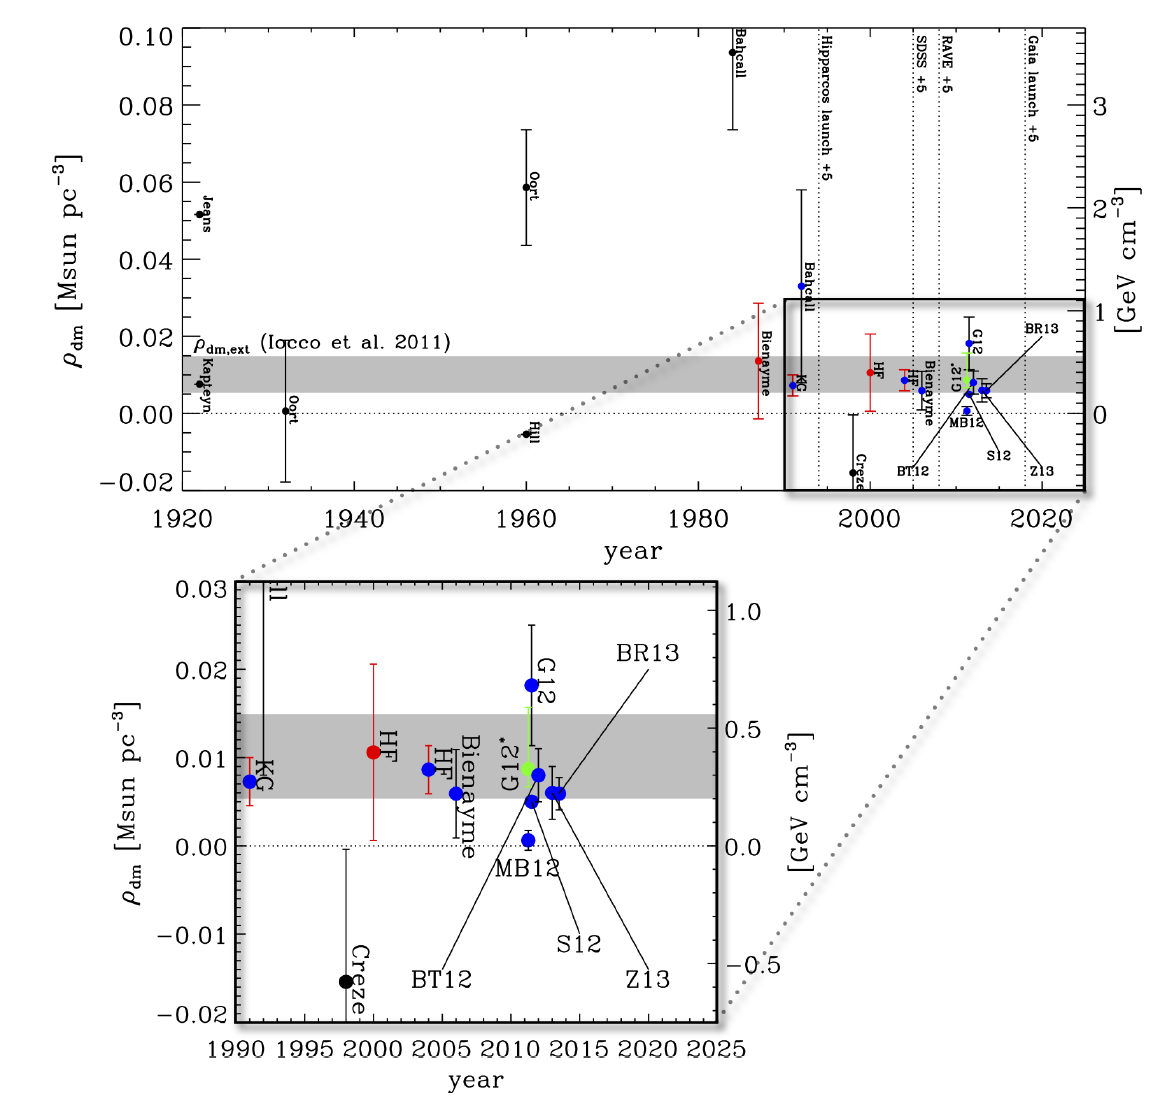
\includegraphics[width=0.7\textwidth]{Century.png}
    \caption{}
\end{figure}


\begin{figure}[h]
    \centering
    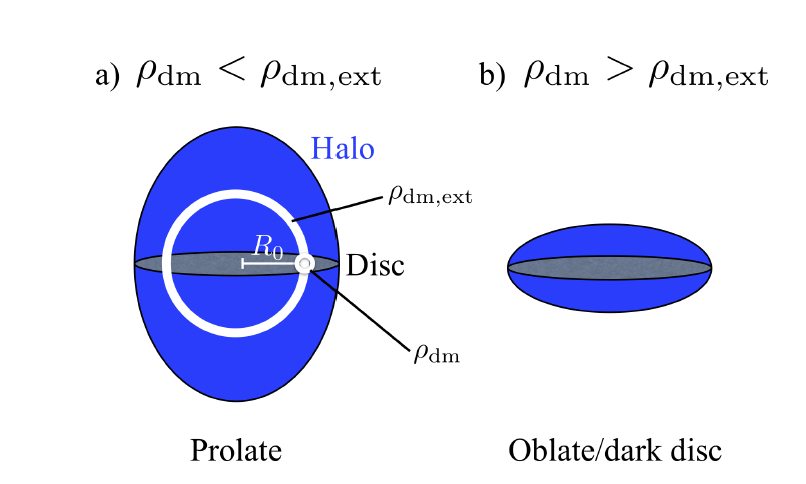
\includegraphics[width=0.7\textwidth]{Halo.png}
    \caption{}
\end{figure}


The local dark matter density, H5
Systematic uncertainties in the determination of the local dark matter density:
https://arxiv.org/pdf/1006.1322.pdf



\subsection{Dark Matter Velocity Distribution \small{\textit{Jelle van Urk}}} \label{DM_Velocity}

\begin{itemize}
    \item minimum \& maximum energy Note: minimum energy might be dependent on elastic/inelastic scattering $v_\text{min}=\sqrt{\frac{m_T E}{2\mu^2_\chi}}$ \cite{Kavanagh:2014rya} for elastic scattering
    \item annual modulation \cite{Undagoitia:2015gya} for more references
\end{itemize}

Velocity Distribution:
Maxwellian distributed, Earth moving through halo, vmin and vmax. Why Maxwellian, shape of halo. 
Or non-Maxwellian, difference in shape distribution. 
As mentioned in section 2.1, the expected recoil rate is necessary 

https://arxiv.org/pdf/1002.1912.pdf
\begin{figure}[h]
    \centering
    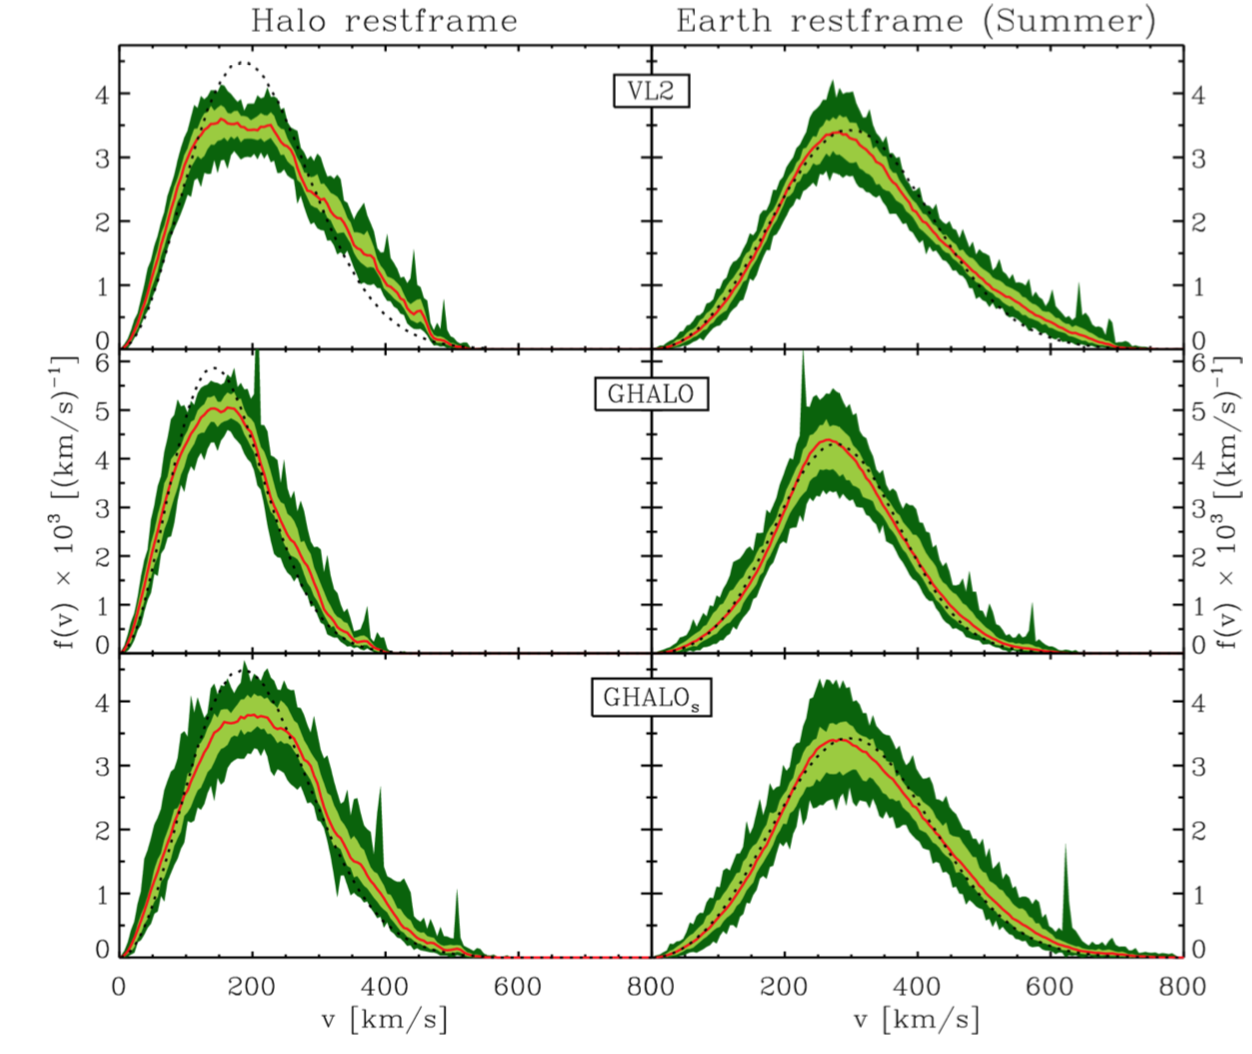
\includegraphics[width=0.7\textwidth]{Vel-dist.png}
    \caption{}
\end{figure}


\begin{equation}
    f(\textbf{v}) = \frac{1}{\sqrt{2\pi}\sigma}e^{-\frac{|\textbf{v}^{2}|}{2\sigma^{2}}}
\end{equation}

% General information about the interaction rate. 
% - General form
% - Form Factor
%   - which is due to the finite size of the nucleus and dependent principally on nuclear radius and recoil energy. This also differs for spin-dependent and spin-independent interactions.
%   - 

% - Velocity distribution
% - Dark matter density distribution
% 

\FloatBarrier
\section{Elastic Scattering}

The two main interaction mechanism between WIMPS and ordinary matter are elastic and inelastic scattering. The idea for elastic scattering of Dark Matter was introduced in 1984 by Goodman \& Witten \cite{Goodman:1984dc} and can produce a nuclear recoil effect necessary for measurement, while the momentum is conserved \cite{Undagoitia:2015gya, Lewin:1995rx}. This can take place in a spin-dependent and spin-independent fashion. 

\begin{figure}[h]
    \centering
    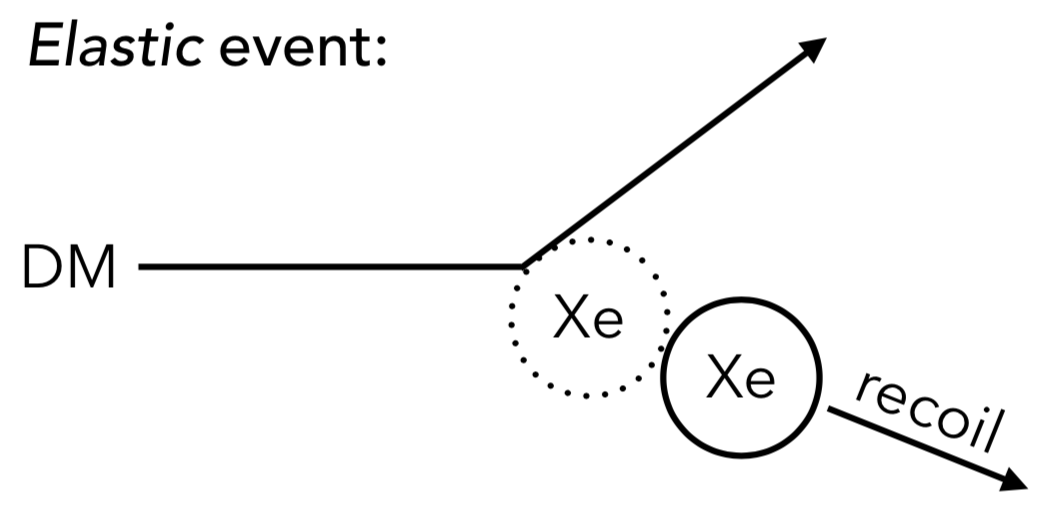
\includegraphics[width=0.7\textwidth]{Elastic_Scattering.png}
    \caption{Elastic scattering of a dark matter of a Xenon atom that recoils due to the collision. Image from \cite{McCabe:2015eia}.}
\end{figure}


\subsection{Spin-independent}

In a WIMP scenario it is expected that spin-independent interactions provide the largest contribution to the effective cross section. This becomes clear if the cross section at zero momentum from equation \ref{Eff_cross} is written out. 

\begin{equation}
    \sigma^\text{SI}_0 = \sigma_{p \chi} \frac{\mu_T^2}{\mu_p^2} \left[Z \cdot f^p + (A-Z) f^n \right]^2
\end{equation}
There is a contribution to the WIMP interaction from the protons and neutrons in the nucleus. In most cases it is assumed that the interactions strength from the protons and neutrons are equal ($f^n = f^p$). This results in a $A^2$ dependence, where A is the atom mass number. 

from the protons and the neutrons in the nucleus 

- Spin-independent
    - Formula
    - fn = fp (isospin violating DM)
    - Strongest interaction expected to see first
    - Implications of target mass on the rate
    - Implications of WIMP on the rate
    - Spin-independent part might vanish depending on the type of particle assumed \cite{Lewin:1995rx}


\subsection{Spin-dependent}

- Implementation into the cross section

- Spin-dependent
    - Formula
    - Depends on average spin n \& p and on the spin quantum number
    - Not as strong
    - Effective-field theory currents for the coupling (an \& ap)


\FloatBarrier
\section{Inelastic Scattering}

Another possible interaction channel is inelastic scattering with three different, but similar outcomes: the nucleus \cite{Ellis:1988nb}, an electron \cite{Starkman:1994gf}, or the WIMP \cite{TuckerSmith:2001hy, TuckerSmith:2004jv, Miao:2013sqa} can be excited in a collision. 




\subsection{WIMP excitation}

The latter mechanism provides an explanation for discrepancies between DAMA \cite{Finkbeiner:2009ug} and CDMS \cite{Ahmed:2008eu} measurement results \cite{Chang:2008gd} and would suppress or even forbid elastic scattering in the detector. This mechanism has been experimentally constraint by the XENON \cite{Aprile:2011ts}, CDMS \cite{Arrenberg:2011zz}, and ZEPLIN \cite{Akimov:2010vk} collaborations. 

\subsection{Nuclear excitation}

The excitation of the nucleus and following de-excitation can be induced by odd mass nuclei \cite{Baudis:2013bba}. Since natural xenon contains odd and even isotopes, experiments using xenon can probe both elastic and inelastic scattering \cite{McCabe:2015eia}. The XENON100 and XMASS collaborations have set upper limit on this spin-dependent inelastic nucleon-WIMP interaction to $3.3 \times 10^{-38}$ cm$^2$ \cite{Uchida:2014cnn, Aprile:2017ngb}. If this interaction is detected, it provides proof for the spin-dependent nature of the WIMP-nucleon interaction. 

\subsection{Electron excitation}

It is also possible for low mass, sub-GeV, WIMPs to recoil off an electron ionizing the atom \cite{Essig:2011nj}. This allows for the probing for low mass dark matter particles as long as electron and nucleon scattering can be distinguished. Over the years several interaction constraints have been set \cite{Essig:2012yx,Essig:2017kqs, Agnes:2018oej,Agnese:2018col,  Crisler:2018gci}


Besides these interaction mechanisms, new ideas and particles have been introduced \cite{TuckerSmith:2004jv,Foot:2013uxa, Undagoitia:2015gya, Bramante:2016rdh} as the dark matter particle. 
Experiments have constraint their possible masses and cross sections \cite{Agnese:2018col}.

\subsubsection{Interaction rate?}

\newpage
\FloatBarrier
\section{Experiments \small{\textit{Peter Bosch}}}
% \begin{itemize}
%     \item Particle created in universe
%     \item Doesn't interact with other particles
%     \item Goes towards Earth
%     \item Comes into detector
%     \item Interacts with e.g. Xenon
%     \item Electrons ejected from collision
%     \item Drifted to detector
%     \item Detector gives signal
% \end{itemize}
Several experiments are operational to detect dark matter directly. In this section the working principle of these detectors, the current experiments and the experiments planned for in the future are discussed.
\subsection{Working principle}
Some of the WIMPs in the universe is directing towards Earth. It is barely interacting with ordinary matter and will reach Earth. There it goes through the atmosphere (without interacting). At the surface it is still not interacting and comes into the underground observatories. At these observatories detectors are placed in big tanks of water to prevent other particles to enter the detector. The used detectors are Time Projection Chambers (TPCs) \cite{Akerib:2015gmi}. The WIMP is interacting with the molecules in the TPC. Some light is created and detected with photomultipliers (S1 signal). The electrons created in the interaction are drifted by an external electric field. When reached the top of the detector, lots of photons are created and detected (S2 signal). In this way interactions between WIMPs and the molecules of the TPC can be detected. This is sketched in figure \ref{fig:working}.

\begin{figure}[h]
    \centering
    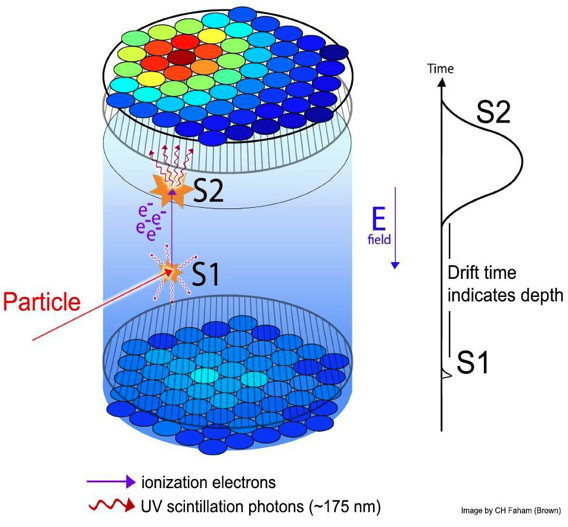
\includegraphics[width=0.7\textwidth]{Principle3.png}
    \caption{Working principle of a DM detector \cite{Akerib:2015gmi}.}
    \label{fig:working}
\end{figure}

With this process, the cross section of the interactions of WIMPs and the molecules of the TPC can be determined. So far, only upper limits of the cross section are found in several experiments (see figure \ref{fig:Sens}). These experiments are covered in section \ref{sec:current_exp}.
\subsubsection{Content TPC}
One can chose the material inside the TPC. Mostly liquid noble-gasses are used. Xenon is the most used noble-gas, although also argon is being used. The advantage of using xenon is that it is sensitive to both spin-dependent and spin-independent interactions \cite{Aprile:2013doa}, it is self-shielding due to a high density (so more xenon can be used for measuring) \cite{Undagoitia:2015gya} and it is stable.

%\hl{``The detector is set up like an enormous bell capable of ringing in response to the lightest tap from a dark matter particle. Nestled within two outer chambers designed to detect and remove contaminating particles lies a chamber filled with 10 tons of liquid xenon. If a piece of dark matter runs into a xenon atom, the xenon will collide with its neighbors, producing a burst of ultraviolet light and releasing electrons.

%Moments later, the free electrons will excite the xenon gas at the top of the chamber and release a second, brighter burst of light. More than 500 photomultiplier tubes will watch for these signals, which together can discriminate between a contaminating particle and true dark matter collisions.''} \cite{PhysOrg}

%Read more at: \href{https://phys.org/news/2017-03-dark-ton.html}{https://phys.org/news/2017-03-dark-ton.html}.
% Plaatje!! :) (Afbeelding 1 van \href{https://www.symmetrymagazine.org/image/april-2012-dark-matter-underground}{Symmetry magazine}, afbeelding 2 van \href{https://phys.org/news/2017-03-dark-ton.html}{Phys.org})

\subsection{Current experiments}
\label{sec:current_exp}
At the moment, several experiments on the direct detection of dark matter are being done. Some of them are discussed here: the PandaX-II detector in Sichuan, China, the LUX detector in South Dakota, USA and the XENON1T detector in Abruzzo, Italy.

\subsubsection{PandaX-II}
\textcolor{red}{P}article \textcolor{red}{and A}strophysical \textcolor{red}{X}enon Detector II (PandaX-II) is a dark matter experiment situated in the region Sichuan in the People's Republic of China. It is a detector with 300 kg of effective liquid xenon target \cite{Liu2015} (more details and latest results in e.g. \cite{Cui:2017nnn}).\\

\begin{figure}[h]
    \centering
    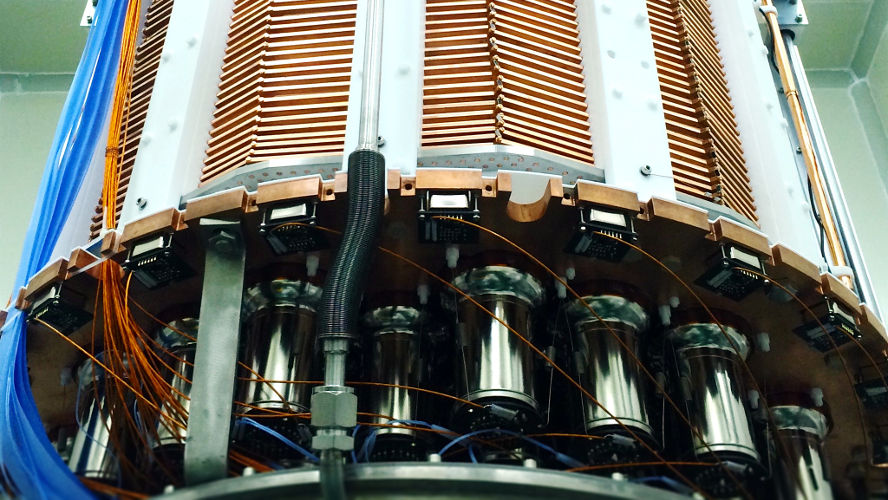
\includegraphics[width=0.9\textwidth]{pandax.jpg}
    \caption{PandaX detector \cite{SJTU}.}
    \label{fig:PandaX}
\end{figure}

\subsubsection{LUX}
The \textcolor{red}{L}arge \textcolor{red}{U}nderground \textcolor{red}{X}enon experiment (LUX) in the Sanford Underground Research Facility near Lead, South Dakota, USA is an 30 million US dollar costing experiment looking for dark matter at 1,480 meters depth \cite{Reich2013}. The latest results are written in \cite{Akerib:2016vxi}. For more details see e.g. \cite{Akerib:2012ys}.

%LUX (Afbeelding van \href{https://physicsworld.com/a/dark-matter-constraints-tightened-after-lux-no-shows/}{Physics World})\\

\begin{figure}[h]
    \centering
    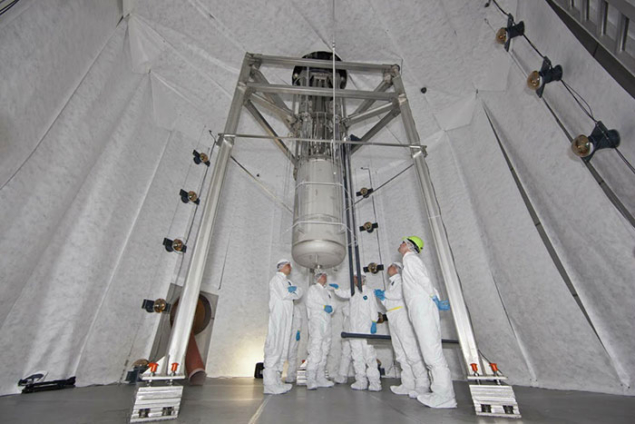
\includegraphics[width=0.9\textwidth]{lux.jpg}
    \caption{LUX detector \cite{PhysWorld}.}
    \label{fig:LUX}
\end{figure}

\subsubsection{XENON1T}
In the Gran Sasso d'Italia - a mountain massive in Southern Italy - several scientific experiments are being done. One of them is the XENON1T dark matter detector. 1.3 tonne of liquid xenon is used to take the latest data \cite{Aprile:2018dbl}. Currently, it is the most sensitive dark matter detector (see figure \ref{fig:Sens}). It set the upper limit for the WIMP-nucleon spin-independent cross section at WIMPs with mass $m_\chi =30\ GeV/c^2$ and $\sigma_\chi^{m=30\ GeV/c^2}<4.1\times 10^{-47}\ cm^2$.
%(Afbeelding van \href{http://www.physics.purdue.edu/darkmatters/xenon1t/?tag=xenon1t}{Perdue University})

\begin{figure}[h]
    \centering
    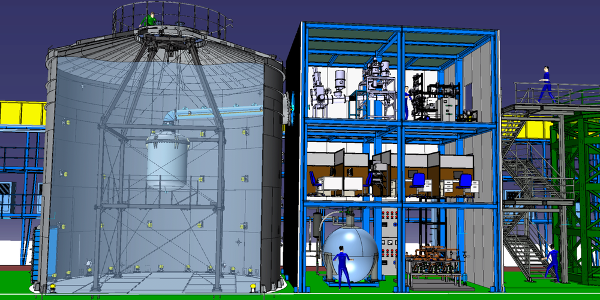
\includegraphics[width=0.9\textwidth]{Xenon1T.png}
    \caption{XENON1T detector \cite{Perdue}.}
    \label{fig:XENON1T}
\end{figure}

\subsubsection{DarkSide}
Next to the XENON1T experiment the DarkSide experiment is running in the Gran Sasso National Laboratory. This is a direct dark matter detector with TPCs based on argon \cite{Agnes:2015ftt, Agnes:2018mon, Edkins:2017qct}. This detector is a few orders of magnitude less sensitive than the detectors with xenon-based TPCs (see figure \ref{fig:Sens}).

%Latest results $\sigma_\chi^{M>6\ GeV/c^2}<4.1\times 10^{-47}$ cm$^2$ \cite{Aprile:2018dbl}.

\begin{figure}[h]
    \centering
    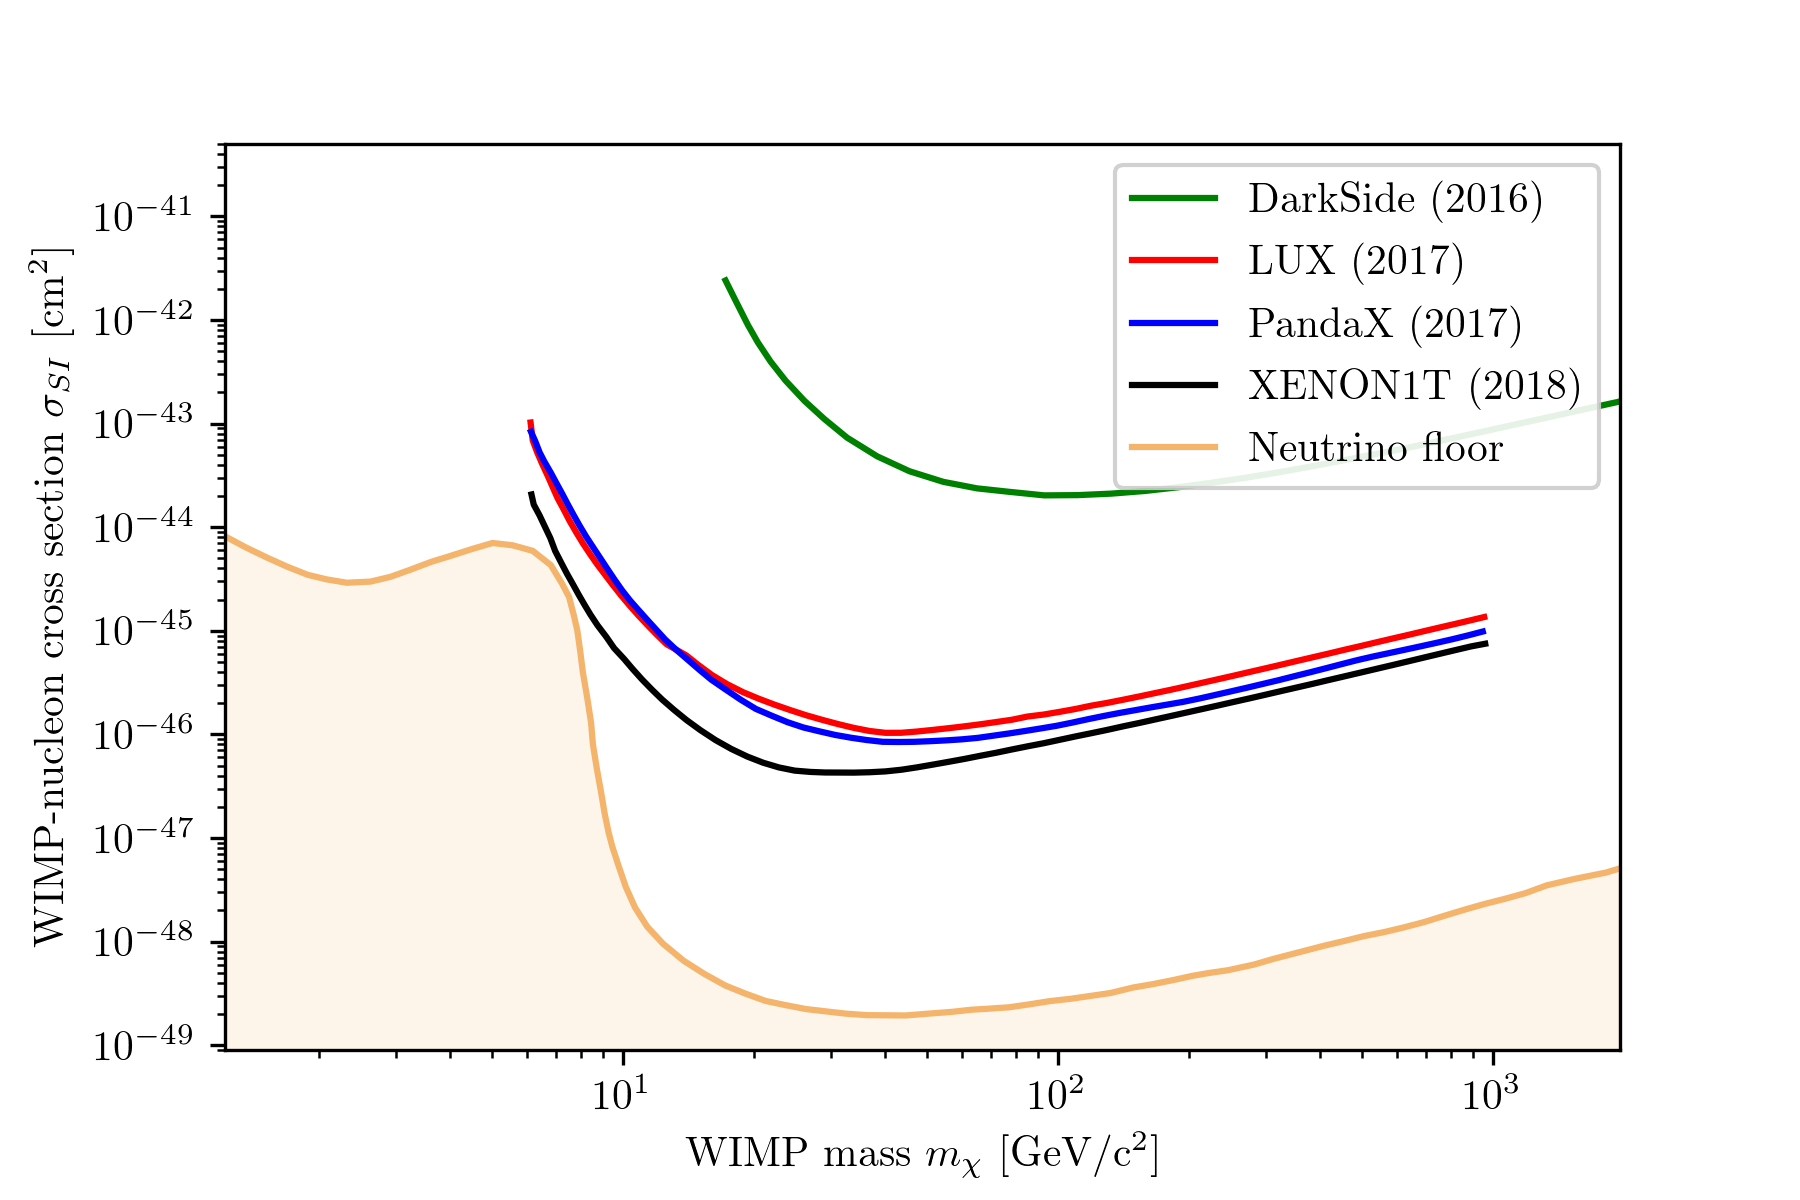
\includegraphics[width=0.7\textwidth]{Sens_plot_floor.png}
    \caption{Sensitivity plot. Data from DarkSide \cite{Agnes:2015ftt}, PandaX \cite{Cui:2017nnn}, LUX \cite{Akerib:2016vxi}, XENON1T \cite{Aprile:2018dbl} and floor \cite{Liu:2017drf}.}
    \label{fig:Sens}
\end{figure}

\subsection{Future experiments}
In the search for dark matter particles one tries to bring down the sensitivity curves (as in figure \ref{fig:Sens}). This is being done with upgrades of existing experiments and building new detectors. Some of them are discussed in this section.

\subsubsection{XENONnT}
The XENON collaboration is working on XENONnT as upgrade of the XENON1T experiment. It is going to be a 5.9 tonne sister of the XENON1T detector \cite{Aprile:2018dbl}. The planning is to be running in 2019 \cite{APPEC}.
%XENONnT ready 2019 (https://science.purdue.edu/xenon1t/)

%\subsubsection{PandaX-30T}
%PandaX-30T

\subsubsection{DARWIN}
DARWIN is a new to build dark matter detector. DARWIN stands for \textcolor{red}{Dar}k matter \textcolor{red}{WI}MP search with \textcolor{red}{N}obble liquids. It will mainly search for WIMPS until the neutrino floor is reached (for the neutrino floor, see section \ref{sec:floor}) \cite{Aalbers:2016jon}. Also research on axions, the low-energy solar neutrinos and galactic supernovae will be preformed.
%DARWIN (https://arxiv.org/abs/1606.07001)

\subsubsection{LZ}
LZ is a combination of \textcolor{red}{L}UX and \textcolor{red}{Z}EPLIN (\textcolor{red}{Z}on\textcolor{red}{e}d \textcolor{red}{p}roportional scintillation in \textcolor{red}{li}quid \textcolor{red}{n}oble gases). It's currently being built in the Sanford Underground Research Facility. See for more (technical) information \cite{Akerib:2015cja,Mount:2017qzi}.


 

\FloatBarrier
\section{Neutrino floor \small{\textit{Peter Bosch}}}
\label{sec:floor}
In dark matter direct detection experiments, one always tries to bring down the sensitivity of interaction in the detector. At a certain moment interactions of neutrinos can not longer be neglected. Although neutrinos have a very small cross section, they do interact. So one will measure the neutrinos in the detector. This is called the neutrino floor. In figure \ref{fig:Sens} the neutrino floor is given. The yellow solid line is the place where one interaction has taken place. So beneath this line, interactions with neutrinos can become a problem. In this section we will go into the neutrino floor and how to go beneath it.

\subsection{Origin of neutrinos \small{\textit{Peter Bosch}}}
As said before neutrinos are interacting inside the detectors. These neutrinos are coming from several sources. The three main sources are
\begin{enumerate}
    \item the sun,
    \item the atmosphere and
    \item supernovae.
\end{enumerate}
Also some other small sources are contributing as neutrino source. All these sources are discussed here.
\subsubsection{Solar neutrinos}
\begin{itemize}
    \item Sun reactions
    \item In some reactions neutrinos produced
    \item Neutrinos go through rest sun
    \item Some go to Earth
    \item Go through atmosphere
    \item Get into detector
    \item Interactions find place
\end{itemize}

\subsubsection{Atmospheric neutrinos}
\begin{itemize}
    \item Particle created in universe (Cosmic ray)
    \item Interaction in outer atmosphere
    \item New particles decay
    \item Cascade of particle interactions/decays
    \item Neutrinos created in cascade
    \item They go through atmosphere and interact in detector
\end{itemize}

\subsubsection{Supernovae neutrinos}

\subsubsection{Other neutrinos}
Earth and nuclear

\subsection{A fundamental limit \small{\textit{Max Briel}}}
\textbf{Max}



\subsection{Continue searching? \small{\textit{Jelle van Urk}}}
\textbf{Jelle}
Direct detection experiments are improving in size and sensitivity for the past couple of years. This means that in the nearby future we will probably reach the neutrino floor, explained in the previous section. This will make the detection for WIMPs even harder, because the scattering interaction events of neutrinos in the detector can be equivalent to a WIMP interaction. Therefore  it's important to understand if it's possible to distinguish the neutrino background events from the dark matter particles. One important step is to better understand the theoretical estimation of the neutrino fluxes. As well as a better measurement to distinguish the different neutrinos entering the detector. 

\subsubsection{Directional experiments}
As described before, most neutrinos are incident from the Sun \cite{Billard:2013qya}. This gives a good opportunity to distinguish them from WIMPs, as the directional signal for these neutrinos would probably be completely different. New experiments are being developed which enable the possibility to measure the incoming direction of WIMPs \cite{Ahlen:2009ev}. 

\subsubsection{Annual modulation}
The DAMA/NaI and DAMA/LIBRA experiments were the first experiment that claimed to have found dark matter \cite{Freese:2012xd}. These results showed an annual modulation of the interaction events which was the highest in June (see figure ...).
\begin{figure}[h]
    \centering
    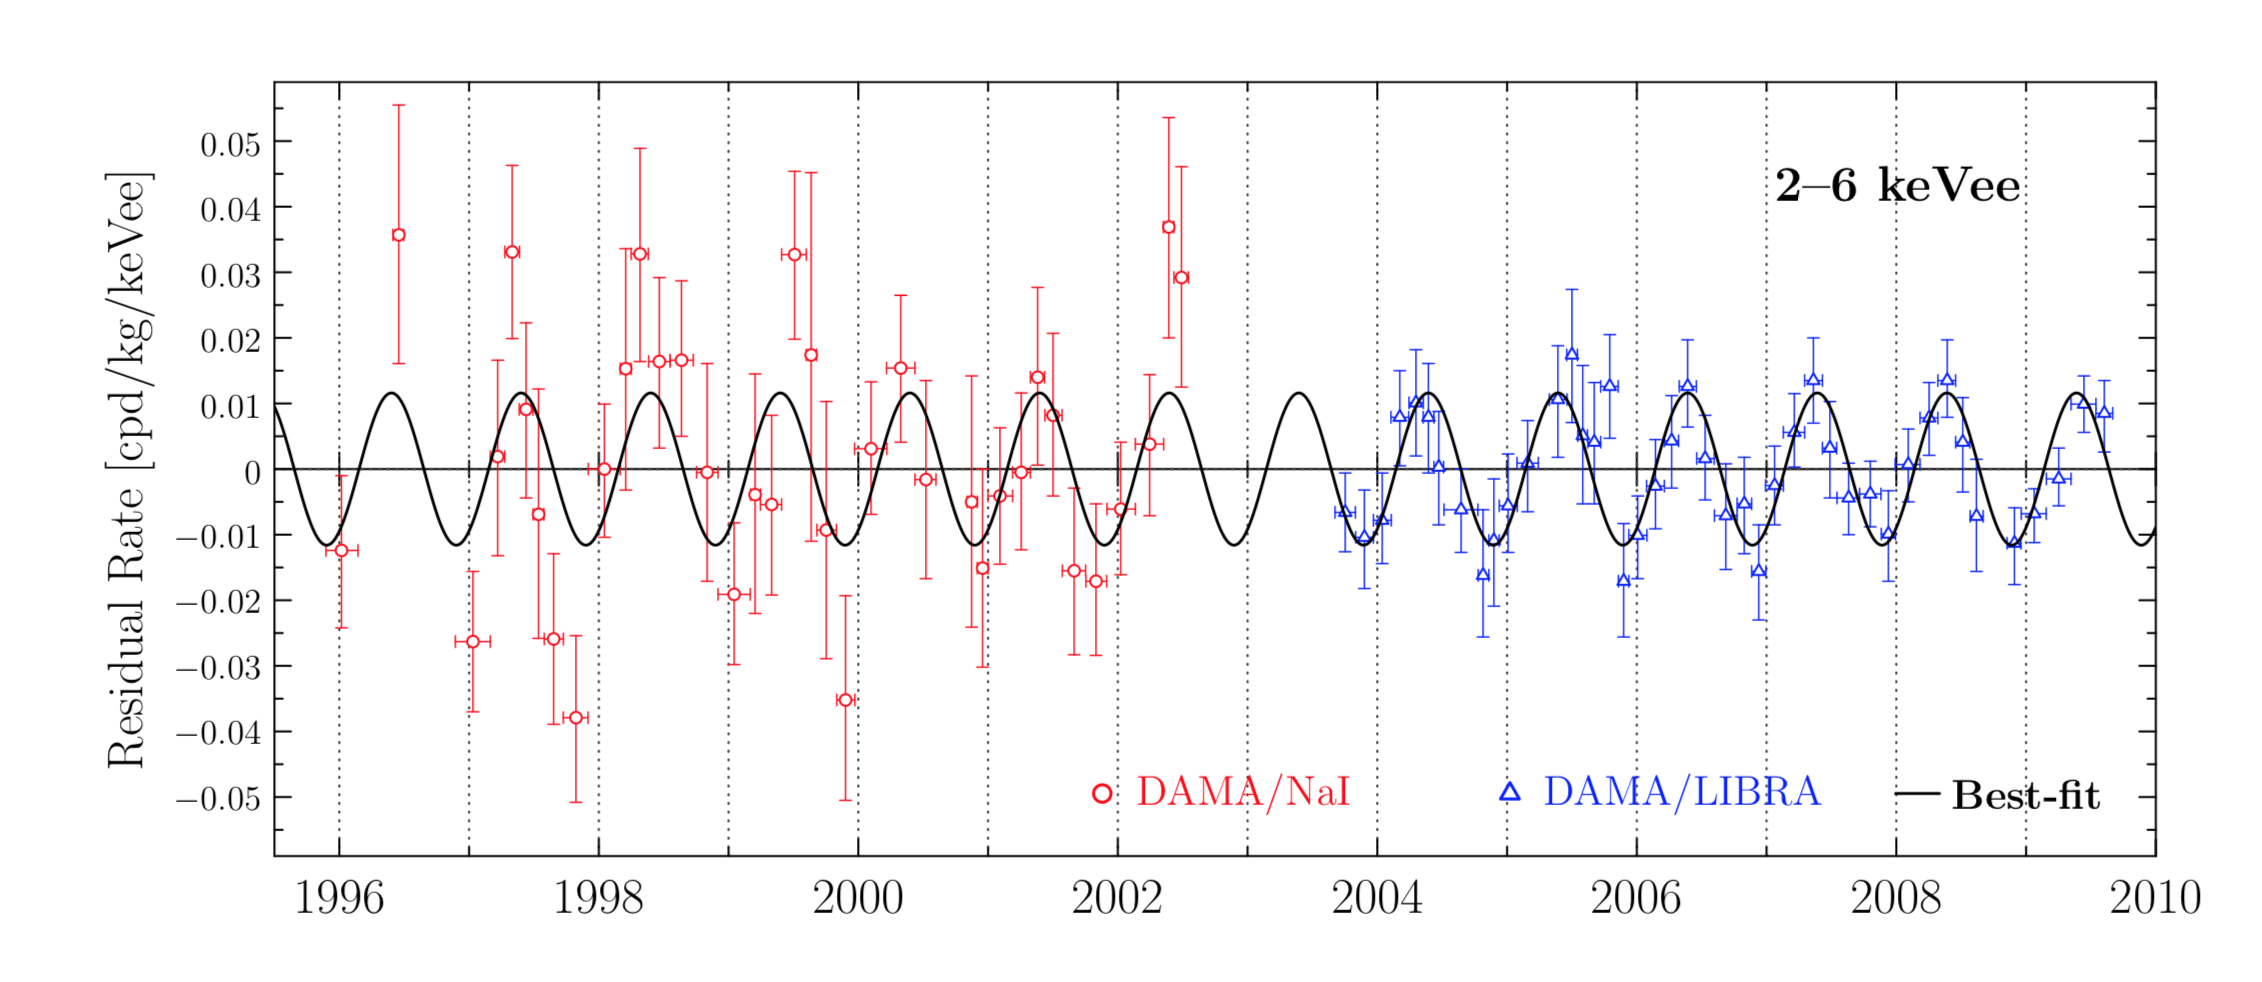
\includegraphics[width=\textwidth]{Annualmodulation.png}
    \caption{}
\end{figure}

\FloatBarrier
\subsubsection{Extraction of neutrino background}
Besides different incoming directions and annual modulation of WIMPs and neutrinos, there will always be some neutrino scattering events which will be similar to those of WIMPs. Therefore it is useful to investigate the how a neutrino only distribution would look like, thus a reconstruction of the neutrino background. 

In the left graph of figure ... you can see a simulated distribution of neutrinos in the range where they could mimic the WIMPs. This simulation is done with Xenon as target nucleus. The legend shows the different origin of neutrinos. The left top of the figure, low mass with high cross section, consist mostly of neutrinos that are incident from the Sun. This is different for atmospheric and diffuse supernova neutrino background (DSNB), which have a higher mass and lower energy (bottom right).
The right graph of this figure shows a accumulation of all the different neutrinos. However, this time a simulation is done with different target nuclei: Xenon, Germanium, Argon, Silicon, Neon and Fluorine. Again, it's obvious that the solar neutrinos (low mass, high cross section) are the most abundant. Xenon and Germanium, which are heaviest of the target nuclei, also show a non-negligible amount of events for atmospheric and SN neutrinos. 
These two graphs show some valuable simulated data. The different target nuclei give slightly different signals. Hence, these target nuclei could be used to distinguish the neutrino background from the WIMPs.
\begin{figure}[h]
    \centering
    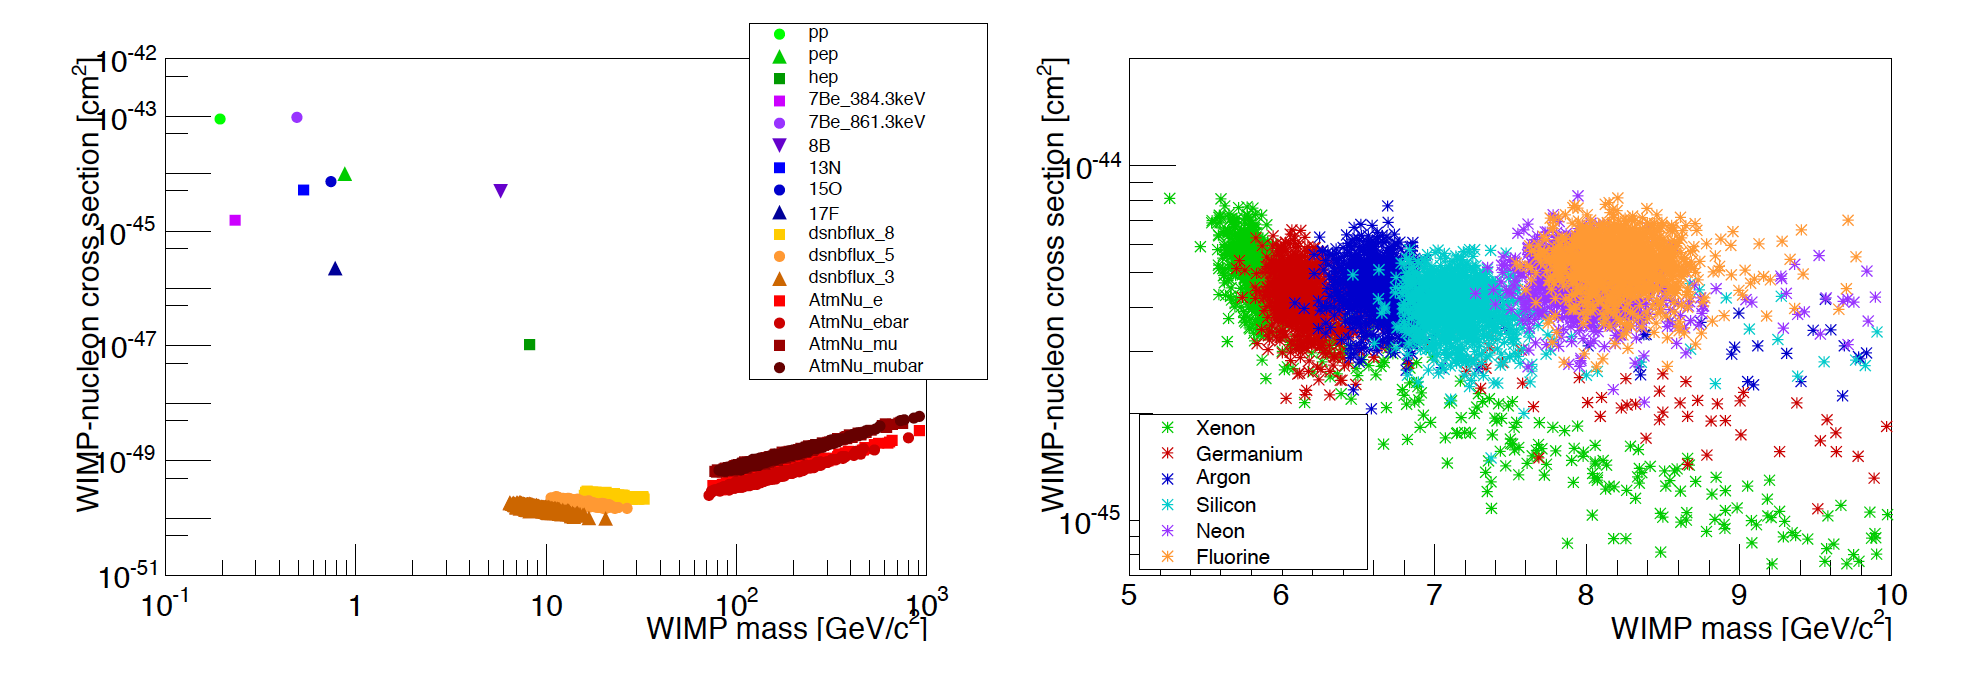
\includegraphics[width=\textwidth]{Neutrinos3.png}
    \caption{\cite{Billard:2013qya}}
\end{figure}







% =============================================================
\FloatBarrier

\
\newpage
\bibliographystyle{unsrt}
\bibliography{refs}

\end{document}

%About nuclear form factor
%http://personalpages.manchester.ac.uk/staff/Sean.Freeman/pc3121/formfactors.pdf

%Reconstruction
%https://arxiv.org/pdf/astro-ph/0703651.pdf